%% question-9.tex
%%

%% ==============================
\subsection{Raffinement du concept d'Instruction}
\label{sec:question9}
%% ==============================

Présenté à la figure \ref{fig:instruction}, le raffinement d'\emph{Instruction} montre qu'une \emph{Instruction} possède trois enfants direct (\emph{Composée}, \emph{Affectation} et \emph{AppelProcédure}).

Le diagramme montre aussi qu'une Instruction est enfant de \emph{Déclaration} (comme présenté dans la figure \ref{fig:declaration}). Cela permet d'éviter d'avoir des tableaux de \emph{Void}.

Sur le diagramme, nous pouvons remarquer la classe \emph{Parametres}, celle-ci a été représentée dans la figure \ref{fig:declaration}.  

\begin{figure}
	\centering
	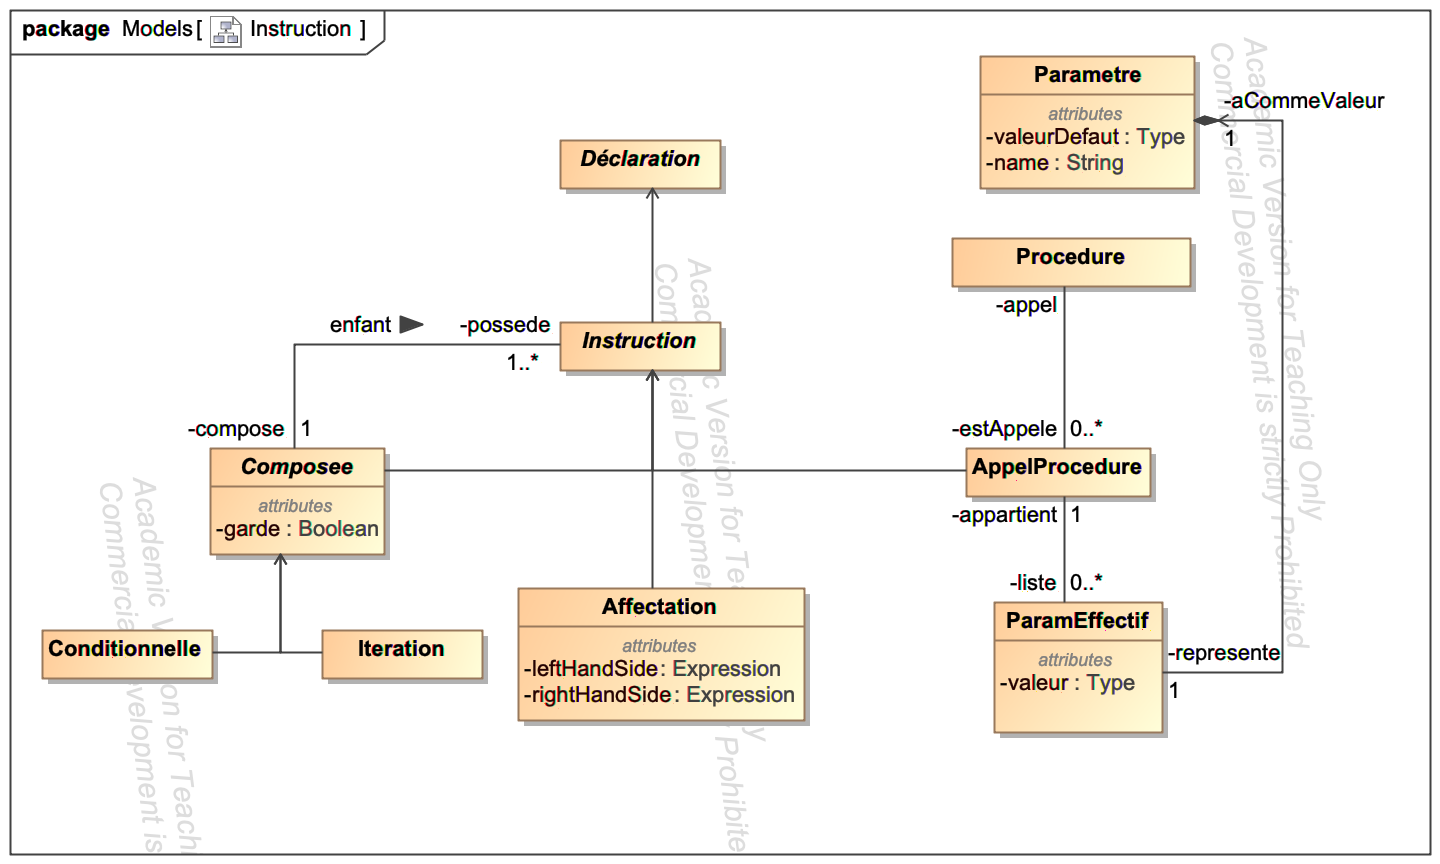
\includegraphics[width=500pt]{assets/class__Instruction}
	\caption{Diagramme de classe d'une instruction}
	\label{fig:instruction}
\end{figure}
